\documentclass[tikz,border=2pt]{standalone}
\usepackage{amsmath,amssymb}
\usepackage{tikz}
\usetikzlibrary{arrows.meta}

\begin{document}
% The open ball B(x0,r): all points strictly closer than r to x0. In the plane with the
% Euclidean distance it is a disc without its rim (dashed).
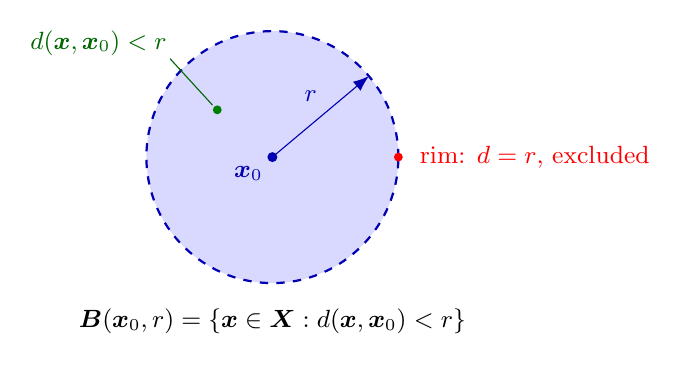
\begin{tikzpicture}[every node/.style={font=\small}]
	\fill[blue!15] (0,0) circle (1.6);
	\draw[blue!70!black, thick, dashed] (0,0) circle (1.6);
	\fill[blue!70!black] (0,0) circle (1.8pt);
	\node[blue!70!black, below left] at (0,0) {$\boldsymbol{x}_0$};
	\draw[-{Latex[length=2mm]}, blue!70!black] (0,0) -- (40:1.6);
	\node[blue!70!black] at (40:0.9) [above left] {$r$};
	\fill[green!50!black] (-0.7,0.6) circle (1.6pt);
	\draw[green!40!black, thin] (-0.76,0.66) -- (-1.3,1.25);
	\node[green!40!black, anchor=south east, inner sep=1pt] at (-1.3,1.25) {$d(\boldsymbol{x},\boldsymbol{x}_0)<r$};
	\fill[red] (1.6,0) circle (1.6pt);
	\node[red, anchor=west] at (1.75,0) {rim: $d=r$, excluded};
	\node[anchor=north] at (0,-1.8) {$\boldsymbol{B}(\boldsymbol{x}_0,r)=\{\boldsymbol{x}\in\boldsymbol{X} : d(\boldsymbol{x},\boldsymbol{x}_0)<r\}$};
\end{tikzpicture}
\end{document}
